\documentclass[a4paper]{article}

\usepackage{ReportTemplate}

\usepackage{setspace}
\usepackage{amsmath}
\usepackage[hidelinks]{hyperref}

\usepackage{graphicx}
\usepackage{subfigure}

\renewcommand{\tt}[1]{\mathtt{#1}}
\newcommand{\bd}[1]{\boldsymbol{#1}}


\title{机器学习工程实践报告:生成模型}
\name{邱一航}
\studentid{520030910155}

\begin{document}

\pagestyle{plain}

\maketitle

\vspace{2em}

\tableofcontents

\newpage

\section{SimSwap的消融实验}

\setcounter{subsection}{-1}
\subsection{实验环境说明}

笔者基于Anaconda进行实验,python版本3.6,CUDA版本v11.1。

运行实验的电脑配置如表\ref{tab1}。

\begin{table}[th]
  \centering
  \begin{tabular}{ c | c c c}
    \toprule
    \textbf{计算单元} & \textbf{型号及性能} & \textbf{数目} & \textbf{容量} \\
    \midrule
    \textbf{CPU} & Intel(R) Core(TM) i5-10300H CPU @ 2.50GHz & 8 & (RAM容量) 16.0GB \\
    \textbf{GPU} & NVIDIA Quadro P620\qquad 算力:6.1 & 1 & 8.0 GB \\
    \bottomrule
  \end{tabular}
  \vspace{0.5em}
  \centering \caption{Configurations of the Computer Executing Experiments}
  \label{tab1}
\end{table}

\vspace{-1.5em}
消融实验的代码及checkpoint见链接\url{https://jbox.sjtu.edu.cn/l/C1fSco}。(如需进行进一步的消融实验,建议重新运行train\_abl.py,不建议直接使用checkpoint;受资源限制,笔者只能设置batchsize为2,checkpoint保存的效果非常糟糕。如果使用更大的batchsize并迭代训练更多轮数,消融实验的结果对比将更明显。)

\subsection{生成模型综述与个人理解}

目前主流的生成模型方法共有四种:对抗神经网络(GAN),变分自动编码器(Variantional Auto-Encoder, VAE),流模型(flow-based models)和传播模型(diffusion models)。

四种方法的大致结构如图\ref{fig1}(下页)所示。

基于GAN的生成模型主要包括判别器和生成器两部分,生成器从某一张图片出发添加一些扰动,生成一张扰动后的图片;而判别器用于判定该图所属的类别。当判别器判断的类别是“该图是真实存在还是电脑生成”,即这张图片是不是很“假”时,训练得到的GAN模型可以从一张图片出发生成另一张看上去很真实的图片。

基于VAE、基于Flow和基于传播模型的生成模型在结构上有相似之处,都可以看作编码和重建两个部分。

对Auto-Encoder,encoder部分对原图进行降维(或称“编码”),得到最核心的表征信息,再通过decoder从表征信息出发重建图像,目的是让原图和重建后的图像尽可能接近,即目标函数是重建误差。朴素AE降维后的潜在空间中数据点的分布可能并不合理,因此在目标函数中加入后验正则项,强迫潜在空间中的数据分布近似特定概率分布,该结构即VAE。

而Flow-based model则通过多个变换G的串联将原本的图像分布(认为是高斯分布)转变为复杂的分布(认为是图像所属类别在特征潜在空间真正的分布),该过程可视为一种“编码”;之后通过一系列逆变换从该分布中的某一点出发生成图像,可视为“重建”过程;flow-based model的目标函数也是减小重建前后图像的误差。

传播模型通过向原图中一点点加噪声来对原图进行改变。从原图出发,经过$T$轮扰动之后图片变为高斯噪声(“前向过程”);而传播模型所做的是想方法从纯高斯噪声重建出原图(“逆向过程”)\cite{overview}。前向过程可以看作是一种“编码”方式,逆向过程则是“重建”的过程。

四种方法的核心都在于:找到所有图像对应的一个潜在空间,不同类别的图像在该空间中有不同的分布;该空间中任意一点都对应了一张图像,而从该点出发生成图像的过程即为“重建”。

\vspace{-1em}
\begin{figure}[htb]
  \centering
  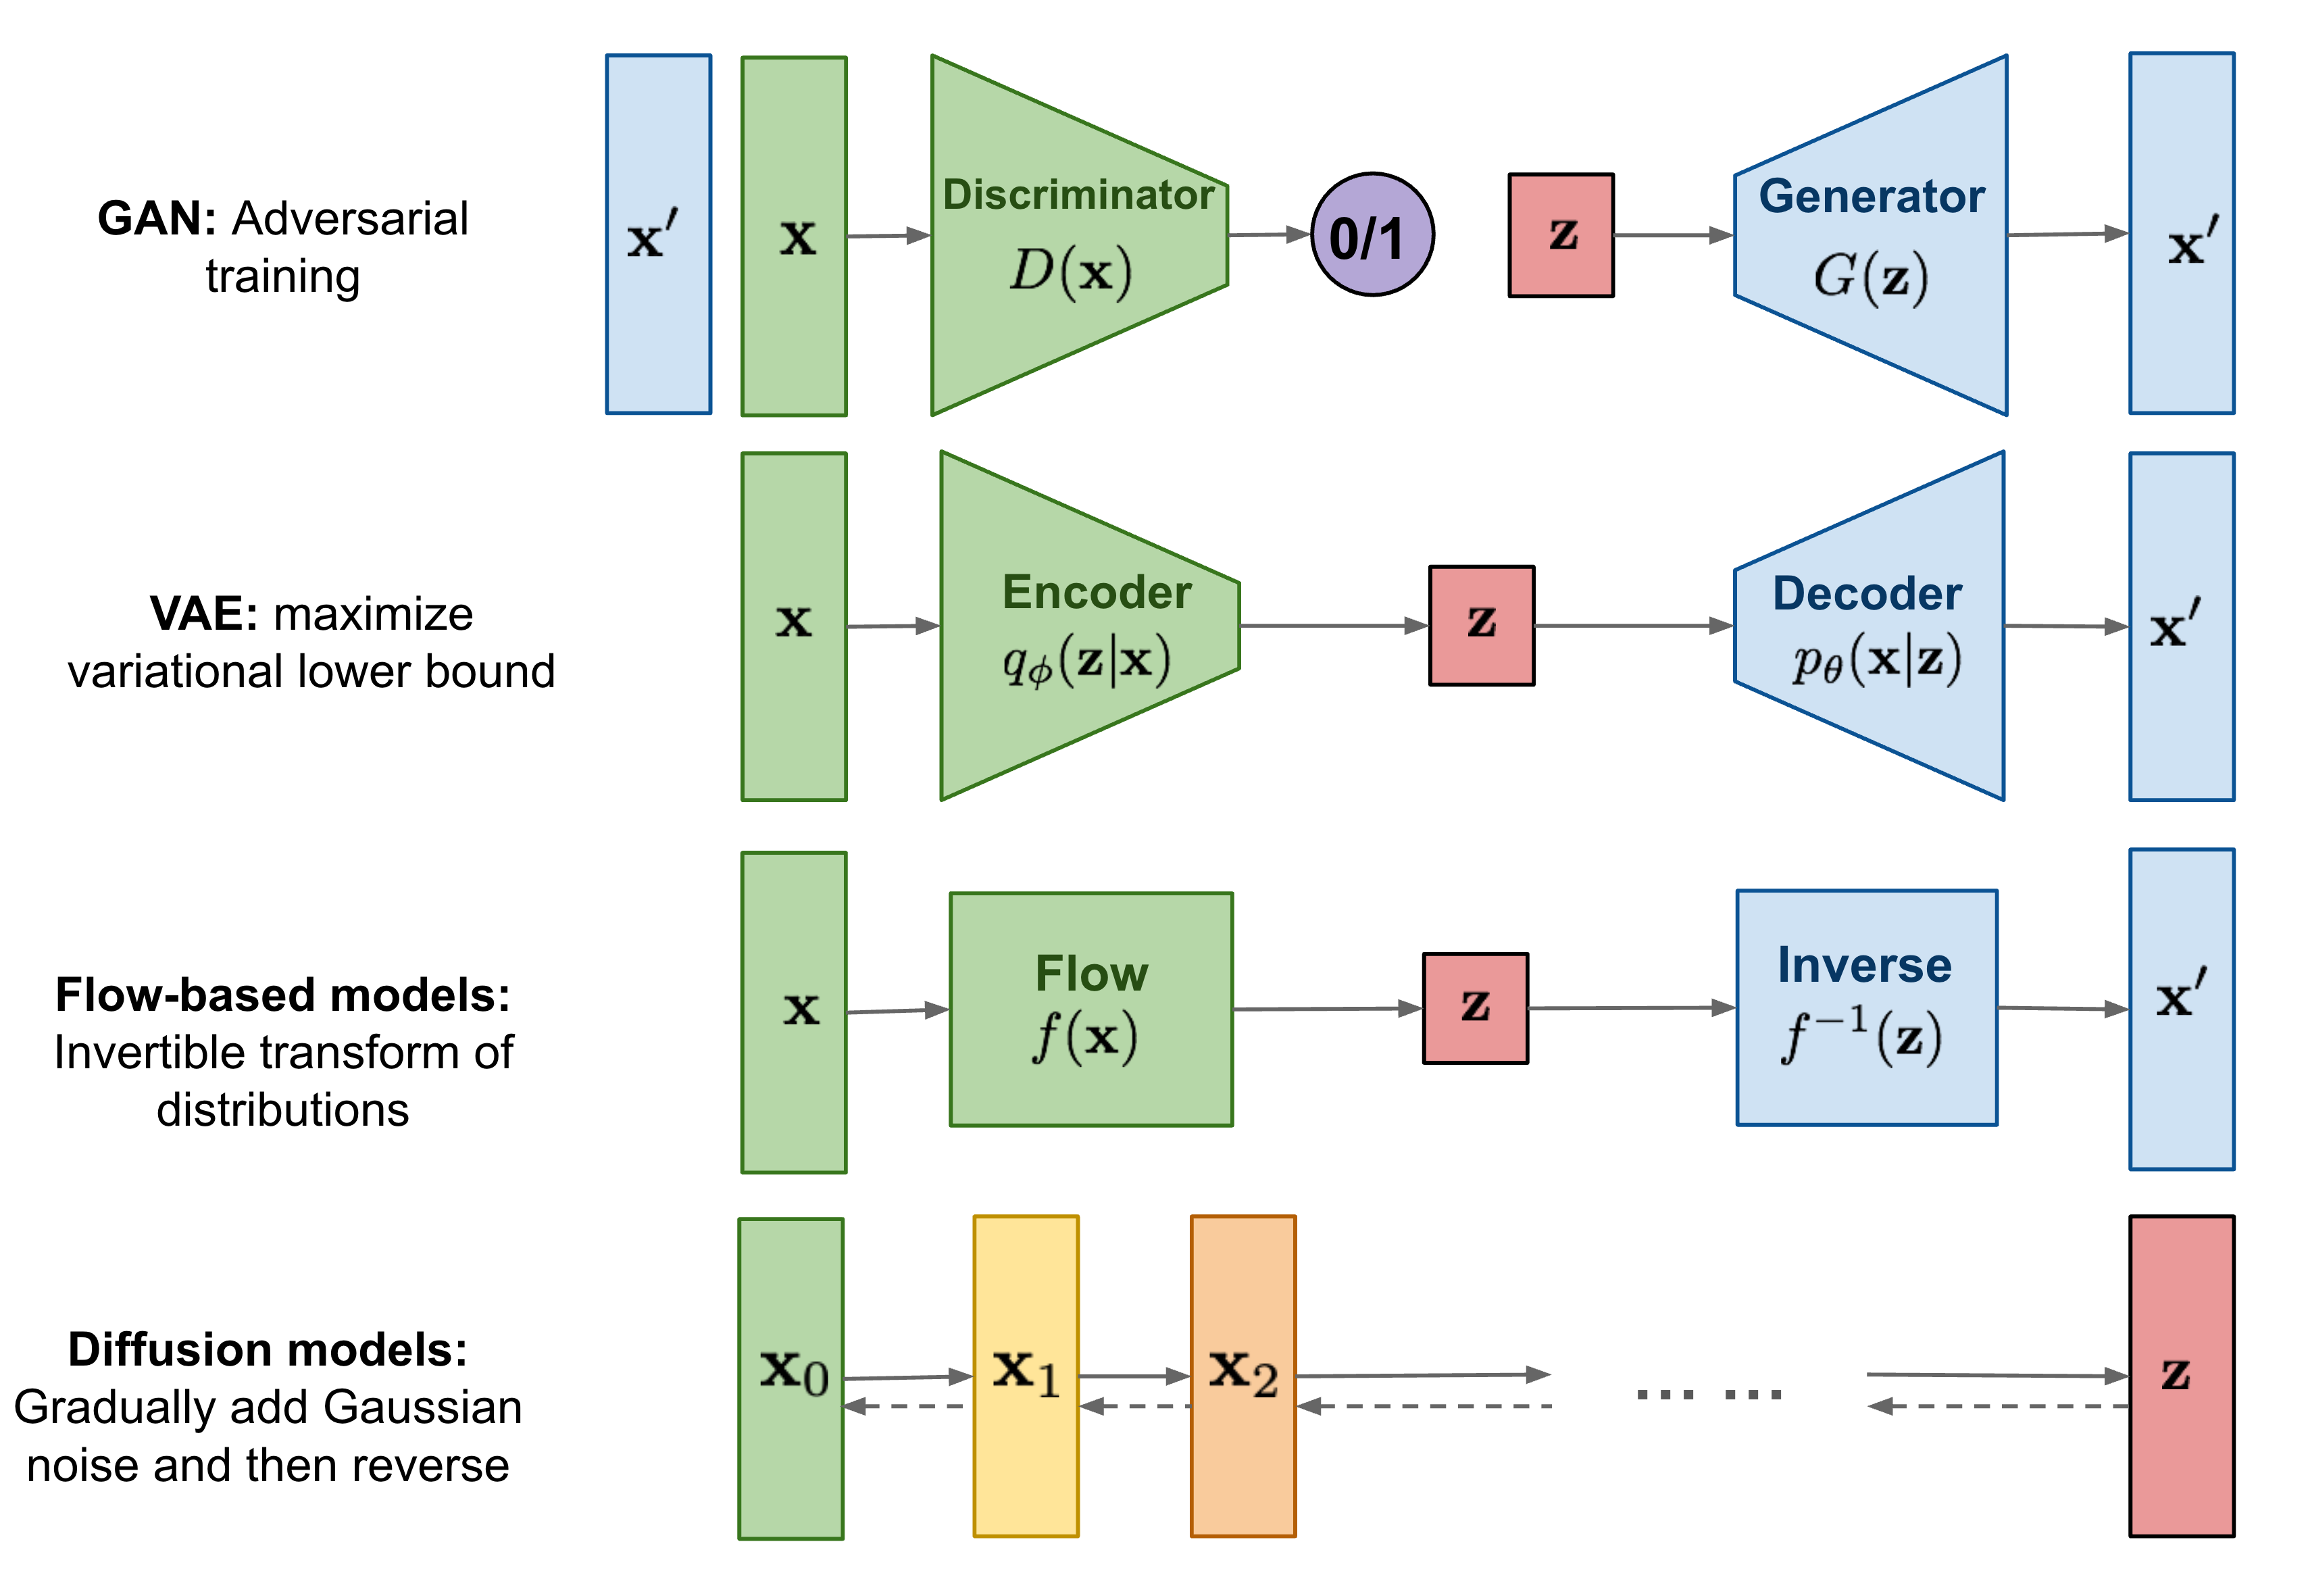
\includegraphics[width=0.95\textwidth]{generative-overview.png}
  \caption{An Overview of Generative Models \cite{overview}}
  \label{fig1}
\end{figure}


\subsection{基于VAE/GAN的换脸模型原理}
朴素的VAE仅仅只是一个生成模型,并不控制生成图像的“方向”,无法生成特定类别的图像。CVAE(条件VAE)将VAE中的概率改为条件概率,从而改变在潜在空间中采样的位置,控制最后生成特定类别的图像。

类似地,GAN模型做的也是从原图出发进行扰动生成另一张图片,无法生成特定类别的图像。将概率换为条件概率后得到的conditional GAN(cGAN)可以生成特定类别的图像。

因此,为实现“换脸”,首先找到换脸源和换脸目标在潜在空间中的位置,向换脸目标的表征中注入换脸源的条件信息(有点类似于图像的风格迁移),再通过重建的方式生成图像。理论上这样做可以实现两张图片不同信息的“融合”,从而实现“换脸”。

\subsection{SimSwap结构简介与消融实验概述}

SimSwap\cite{simswap}的整体结构如图\ref{fig2},该方法结合使用了VAE和GAN。

SimSwap的结构主要分为生成器Generator部分(下面简称Net G)和判别器Discriminator部分(下面简称Net D),大框架类似cGAN-based生成模型。Generator部分采用了cVAE的结构,但在encoder和decoder之间的bottleneck部分提取换脸源的特征信息并注入到换脸目标的特征信息中。最终的loss函数基于生成的换脸结果的特征信息和Encoder提取的换脸源的特征信息构建。
 
\begin{figure}[htb]
  \centering
  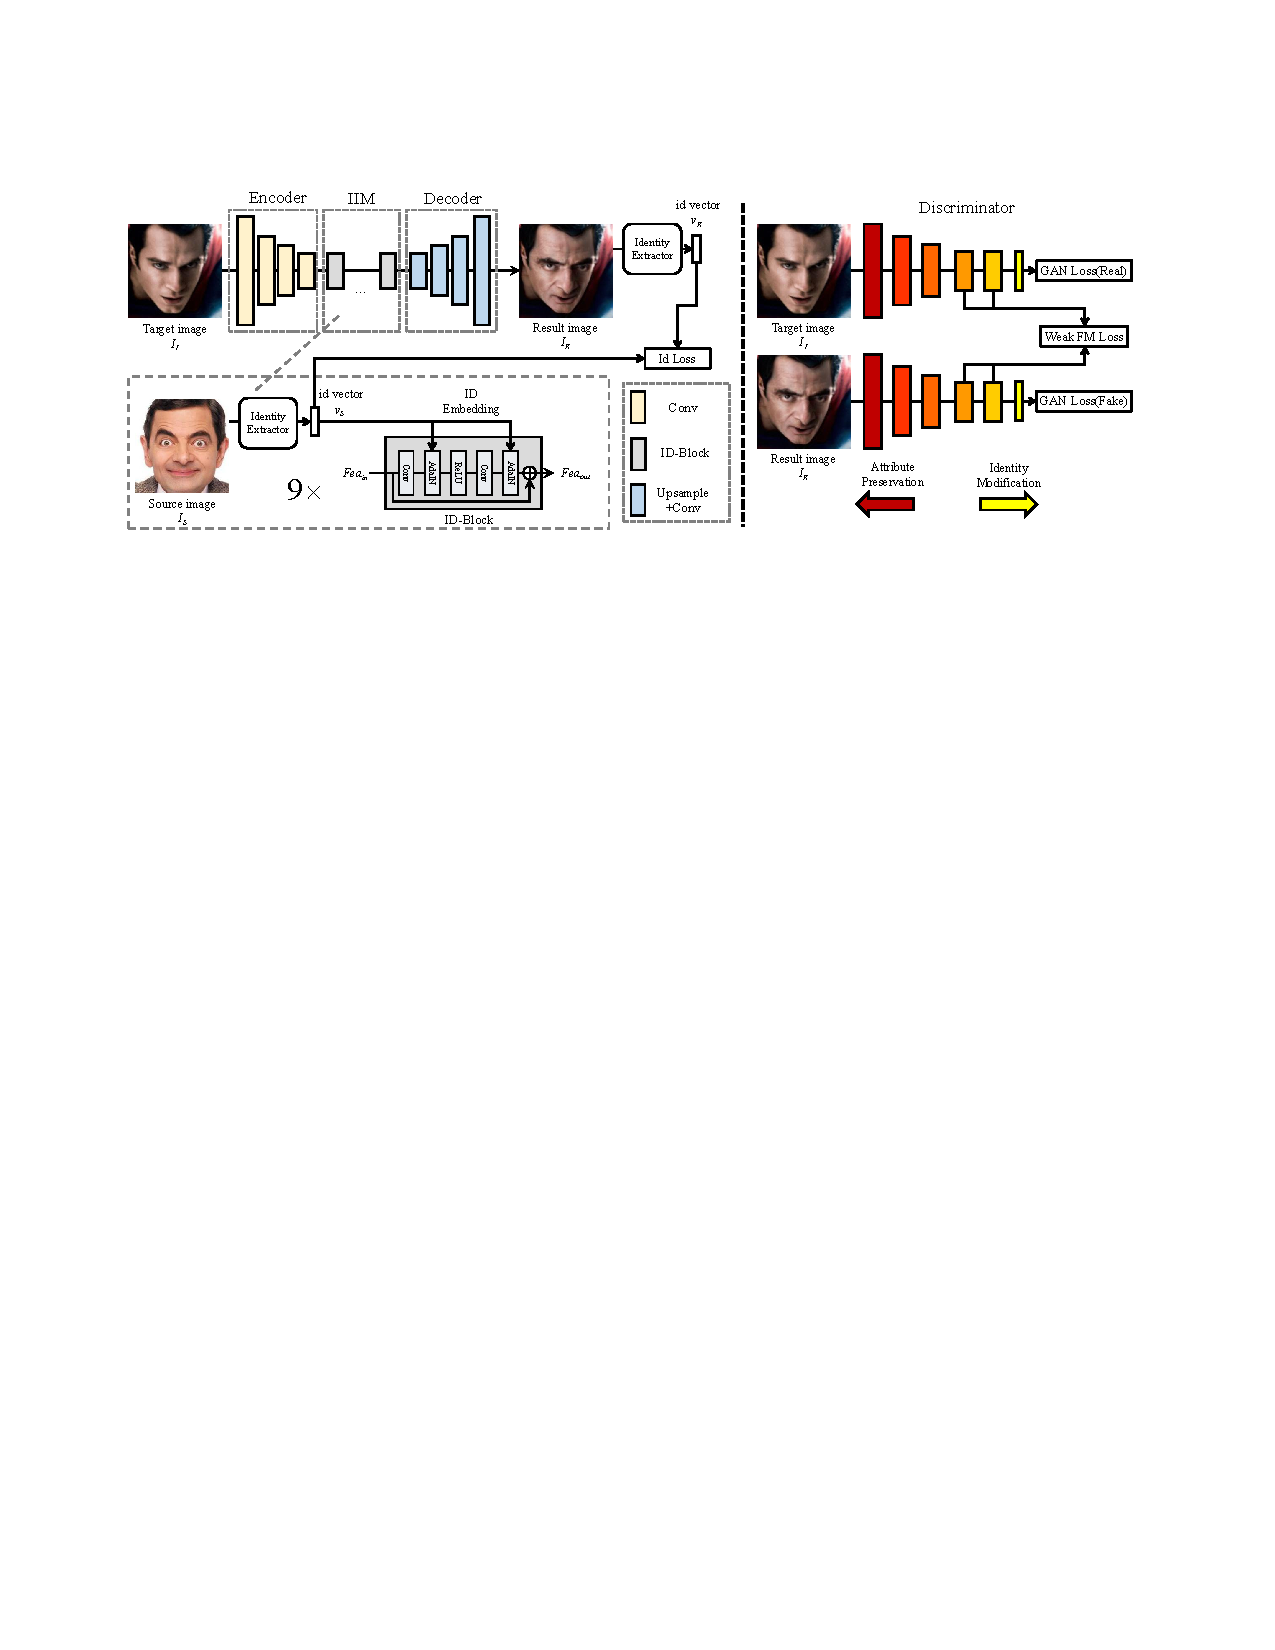
\includegraphics[width=\textwidth]{simswap.pdf}
  \caption{An Overview of SimSwap \cite{simswap}}
  \label{fig2}
\end{figure}

\vspace{1em}
\textcolor{red}{为了进行消融实验,笔者对源代码进行了下列修改:}

\vspace{-0.5em}
\begin{itemize}
    \item 对$\tt{train.py}$进行修改得到$\tt{train\_abl.py}$,新增了ablOnG选项用于指定Net G上消融实验的类型(without\_encoder, without\_bottleneck, without\_decoder)和loss选项用于指定Loss函数中$L_{Recon}$和$L_{wFM}$的范数(L1或L2)。原始的loss函数如下,$L_{Recon}$和$L_{wFM}$采用L1范数:
    
    \vspace{-2.5em}
    \begin{align*}
        \mathcal{L}&=\lambda_{Id}L_{Id} + \lambda_{Recon}L_{Recon} + L_{adv} + \lambda_{GP}L_{GP} + \lambda_{wFM}L_{wFM}
    \end{align*}
    
    \vspace{-1.2em}
    为防止对SimSwap源文件造成影响,笔者备份$\tt{model}$文件夹为$\tt{model\_abl}$文件夹,$\tt{train\_abl.py}$仅使用该文件夹的内容。
    \item 修改了$\tt{model\_abl/fs\_network\_fix.py}$和$\tt{projected\_model.py}$,完成消融实验的实现部分。每个消融实验的具体处理将在下面说明。
\end{itemize}

\subsection{针对SimSwap Net G的消融实验设计}

SimSwap使用的Net G采用VAE的结构,共有encoder、bottleneck、decoder三个部分。笔者分别对三个部分进行消融实验,以验证各个部分的功能和存在的必要性。

受资源限制,笔者只能运行batchSize为2的实验,且仅迭代训练50000次。该条件下训练得到的原始模型分类结果见图\ref{app0}。

\subsubsection{Encoder部分}

SimSwap中,encoder部分为多层卷积层,用于提取换脸目标图片中的特征信息(进行不同区域的划分)。由于encoder的输入和输出并不是相同尺寸,因此笔者将输入图像强行缩放并复制灰度图通道作为原本多个通道的输出,拼接后作为bottleneck部分(即图\ref{fig2}中的IIM部分)的输入。

考虑到输入与输出的图片尺寸并非倍数关系,直接采样会有问题。因此使用bicubic插值(该方法的放大效果优于bilinear)\cite{AI2619}对原图进行插值后,再进行采样得到缩放后的图片。笔者的消融实验代码中也提供了bilinear插值方法的使用说明。

移除encoder部分消融实验得到的换脸结果见附录中图\ref{app1},对比分析见\textbf{1.7}。

\subsubsection{Bottleneck部分}

其实不进行消融实验我们也知道bottleneck部分(IIM)的目的是将换脸源的特征信息注入到换脸目标图像的特征中。因此移除这一部分会导致换脸目标图片无法获得换脸源的具体信息,基本上维持原样。

bottleneck部分的输入和输出是同一结构,因此该部分的消融实验并不需要做特殊处理,直接pass即可。

移除bottleneck(IIM)部分消融实验得到的换脸结果见附录中图\ref{app2},对比分析见\textbf{1.7}。

\subsubsection{Decoder部分}
SimSwap中,decoder部分为多层“bilinear上采样+卷积层”的结构,用于将IIM后得到的特征信息重建为图片。由于decoder的输入和输出并不是相同尺寸,因此该部分的消融实验需要做一些处理。笔者将IIM输出的特征强行放大到要求的生成图片尺寸,并只保留前3个通道的数值。

实际上,在通道数缩减方面笔者有一个相对更好的想法,即\textcolor{red}{将原本的512个通道视为512个维度,或许使用PCA将其降维至3维(3个通道)作为输出效果更好。但考虑到如此大维度数据的PCA需要的时间和计算资源,笔者放弃了这一想法。}

由于输入的特征信息的维数是小于输出图片的尺寸的,因此如何放大会影响最终效果。与\textbf{1.4.1}中相同,笔者这里使用bicubic插值方式进行放大。笔者的代码中也提供了bilinear插值方式的使用说明。

移除decoder部分消融实验得到的换脸结果见附录中图\ref{app3},对比分析见\textbf{1.7}。

\subsection{针对SimSwap Loss的消融实验设计}

SimSwap的Loss设计包括了多项内容:用于判定换脸结果中人脸特征与换脸源特征是否相近的Identity Loss($L_{Id}$)、用于判定换脸结果与换脸目标是否相近的Reconstruction Loss(重建损失,$L_{Recon}$)、GAN判别器的Adversarial Loss和Gradient Penalty Loss($L_{adv}$和$L_{GP}$)和SimSwap新提出的weak Feature Matching Loss(弱特征匹配损失,$L_{wFM}$)。

其中,$L_{Id}, L_{Recon}, L_{wFM}$为Net G上的Loss,$L_{adv}, L_{GP}$为Net D上的Loss。本小节中只对Loss G部分进行消融实验。

    \vspace{-2.2em}
    \begin{align*}
        \mathcal{L}=\mathcal{L}_G+\mathcal{L}_D=\lambda_{Id}L_{Id} + \lambda_{Recon}L_{Recon} + L_{adv} + \lambda_{GP}L_{GP} + \lambda_{wFM}L_{wFM}
    \end{align*}
    
\vspace{-0.5em}
由于时间限制和资源限制,笔者仅完成了对重建损失 $L_{Recon}$和弱特征匹配损失 $L_{wFM}$范数形式的消融实验,将两者原本的L1范数形式更改为L2范数形式。

换用L2范数的$L_{Recon}$和$L_{wFM}$后,消融实验得到的换脸结果见附录中图\ref{fig-loss},对比分析见\textbf{1.8}。

\subsection{未实现的消融实验设计}

笔者仅对SimSwap的Net G部分和部分Loss的范数形式进行了消融实验。SimSwap模型中的net D和loss中各项的不同作用也应当进行消融实验,但限于时间因素和资源因素,笔者并未能完成这部分实验。这里只给出消融实验的想法或代码实现。

\subsubsection{Net D}

SimSwap中判别器部分直接使用了其他模型(EfficientNet\_Lite)的训练结果,并未给出显式的网络结构。因此笔者难以通过代码的方式直接对这一部分进行消融实验。

但为证明该部分使用该模型的必要性,应将这一模型替换为其它图像分类模型进行消融。

\subsubsection{Loss结构}

\textbf{1.5}中仅设计了改变范数的Loss消融实验,未对各个Loss进行消融。实际上,更完整的消融实验应该如下:

\begin{itemize}
    \setstretch{0.9}
    \item $\lambda_{Id}=0.$ 研究Id Loss的必要性。
    \item $\lambda_{Recon}=0.$ 研究重建损失的必要性。
    \item $\lambda_{wFM}=0.$ 研究弱特征匹配损失的必要性。
\end{itemize}

此外,SimSwap的一个核心创新点在于weak Feature Matching Loss(弱特征匹配损失),该损失只对判别器最后几层提取的特征进行了对比。这一创新主要是考虑到换脸结果与换脸目标、换脸源均不同,并不存在“真值”,而判别器前几层提取的特征更“本质”,更有可能是脸部识别相关的特征;最后几层则更像是非人脸相关的特征。

为了研究该损失的必要性还,应该设计以下两个消融实验。

\begin{itemize}
    \setstretch{0.9}
    \item 直接使用Feature Matching Loss替代wFM Loss
    \item 用针对判别器前几层的特征结果使用Feature Mathcing Loss的方式替代wFM Loss
\end{itemize}


\subsection{Net G上消融实验结果}

Net G不同消融实验下各部分Loss的变化情况如图\ref{lossG-G}和图\ref{lossD-G}(均在下页),两者分别为LossG和LossD的变化情况对比。

\subsubsection{LossG: Net G上的整体损失与各部分损失分析}

Loss G由Id Loss、Reconstruction Loss和wFM Loss三部分组成,即

\vspace{-2.2em}
    \begin{align*}
        \mathcal{L}_G=\lambda_{Id}L_{Id} + \lambda_{Recon}L_{Recon} + \lambda_{wFM}L_{wFM}
\end{align*}

\vspace{-0.5em}
由图\ref{lossG}可见,移除decoder部分后,Net G上的Loss居高不下。很显然decoder的移除导致图像的重建结果非常糟糕(这点由换脸结果\ref{app3}也可见),因此损失函数始终较大,结果符合预期。

移除encoder部分后,Net G上的Loss整体而言高于原版本,但依然能够收敛。这证明消融实验中用于替代encoder的缩放操作实际上也可以作为一种“编码”的方式,使整个SimSwap系统能继续工作;但Loss整体偏高也证明了SimSwap系统中设计的多层卷积的encoder具有较为良好的效果。这些结果也符合预期。

\vspace{1em}
下面具体分析各个部分的消融实验对各个Loss的影响。

\vspace{1em}
\textbf{1. Id Loss}。

由图\ref{Id}可见,各个部分的存在与否对Id Loss的影响并不明显。这是由于实验的训练轮数远远没到训练完成的程度,换脸源的特征尚未能完全注入换脸结果中,因此消融实验前后Id Loss的变化较小。同时,从大约40000轮开始,移除了IIM部分后Id Loss的波动范围明显大于其余三者,证明IIM有效地将换脸源的特征信息注入到了换脸结果中。

\begin{figure*}[htb]
\centering

\subfigure[LossG (Total)]{\label{lossG}
    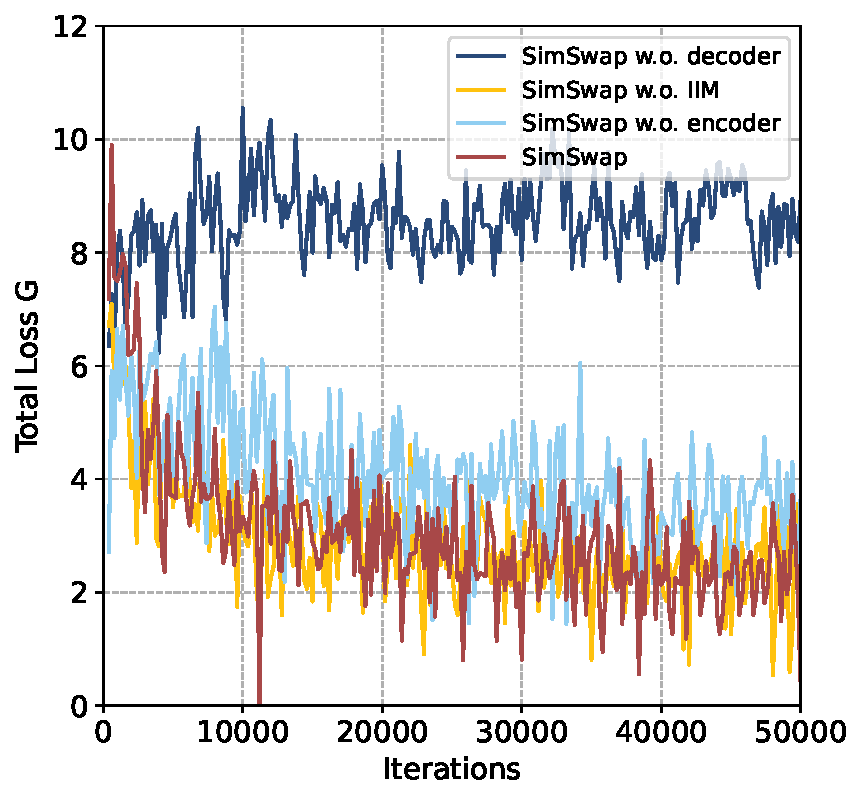
\includegraphics[scale=0.485]{lossG.pdf}
    }
&
\subfigure[Id Loss]{\label{Id}
    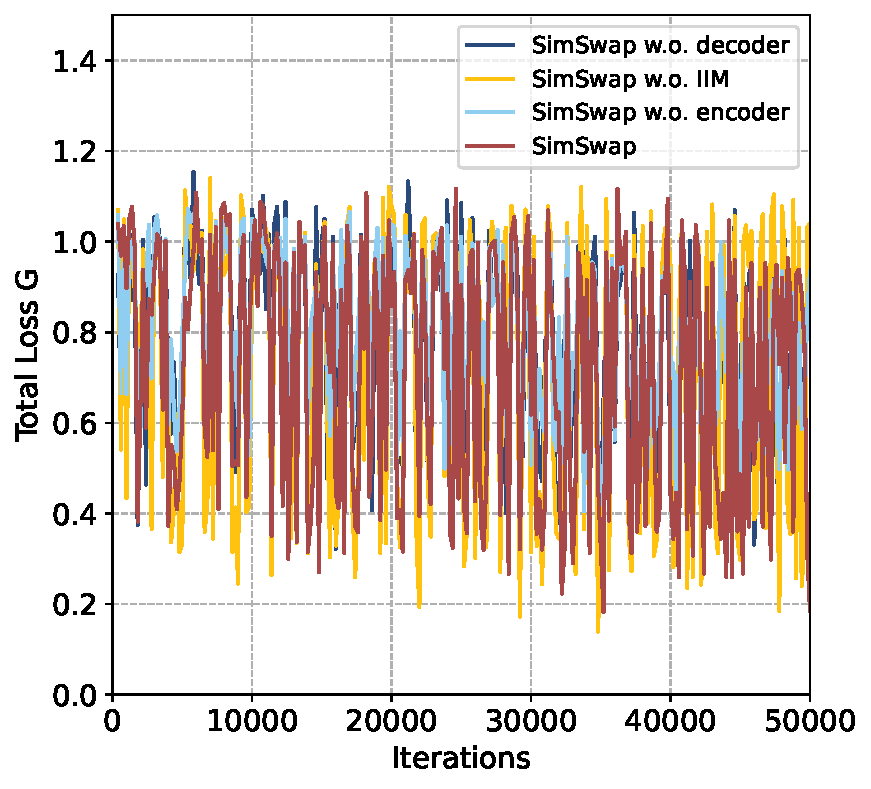
\includegraphics[scale=0.485]{ID.pdf}
    }
\\
\subfigure[Rec Loss]{\label{rec}
    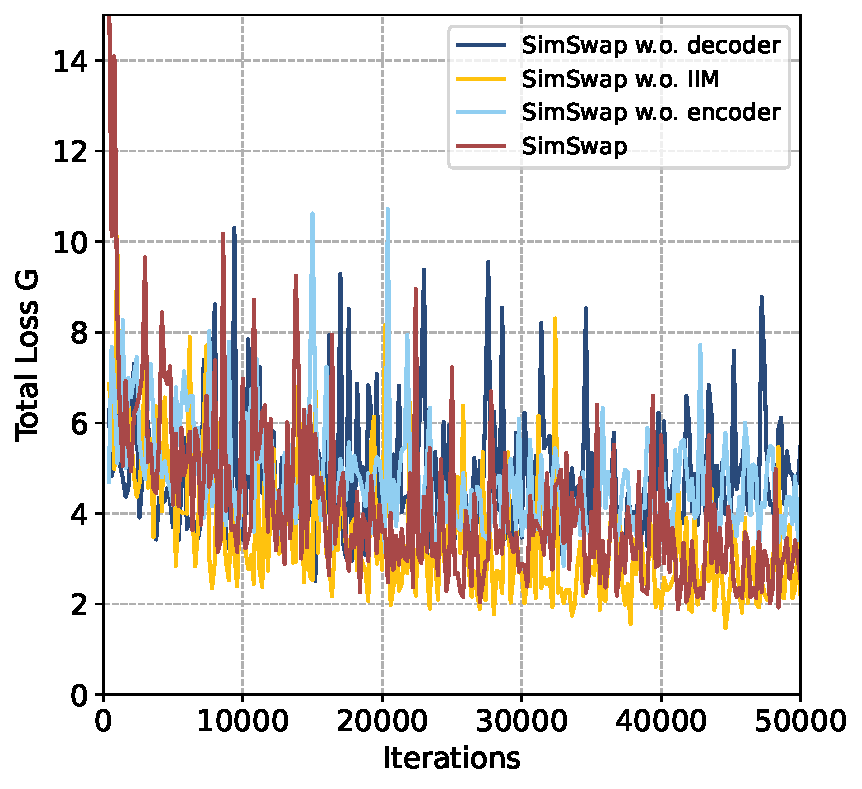
\includegraphics[scale=0.485]{Rec.pdf}
    }
&
\subfigure[wFM Loss]{\label{wFM}
    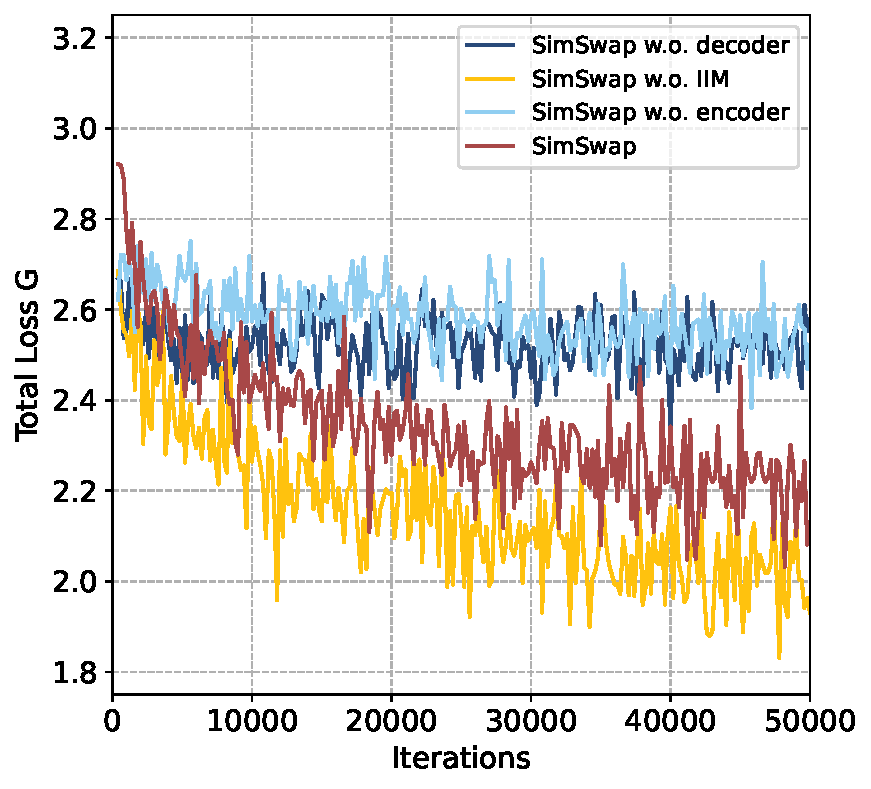
\includegraphics[scale=0.485]{feat.pdf}
    }
\caption{Change of Loss G in Ablation Studies of Net G}
\label{lossG-G}
\end{figure*}

\vspace{-2em}
\begin{figure*}[!htb]
\centering

\subfigure[LossD (Total)]{\label{lossD}
    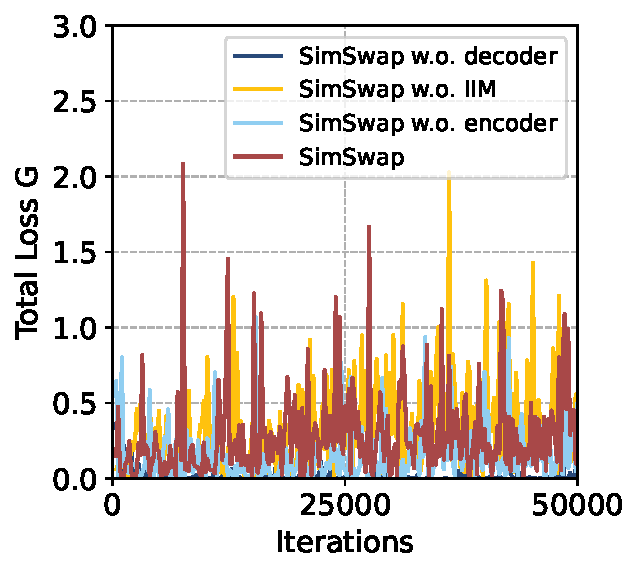
\includegraphics[scale=0.42]{lossD.pdf}
    }
&
\subfigure[D\_fake]{\label{D_fake}
    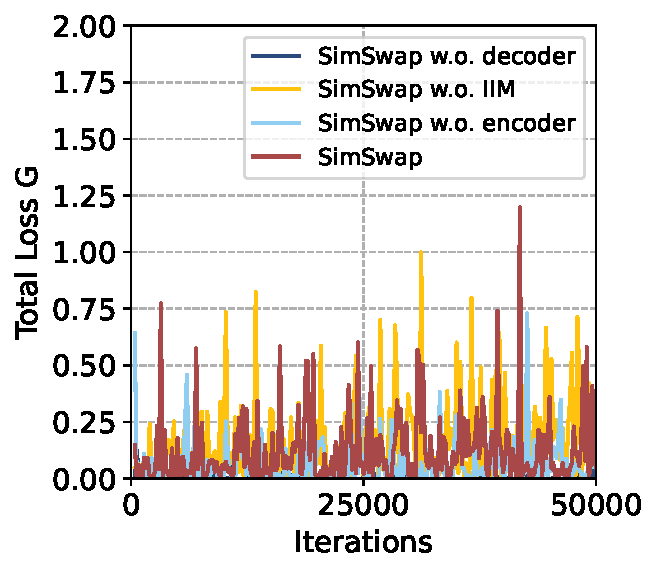
\includegraphics[scale=0.42]{fake.pdf}
    }
&
\subfigure[D\_real]{\label{D_real}
    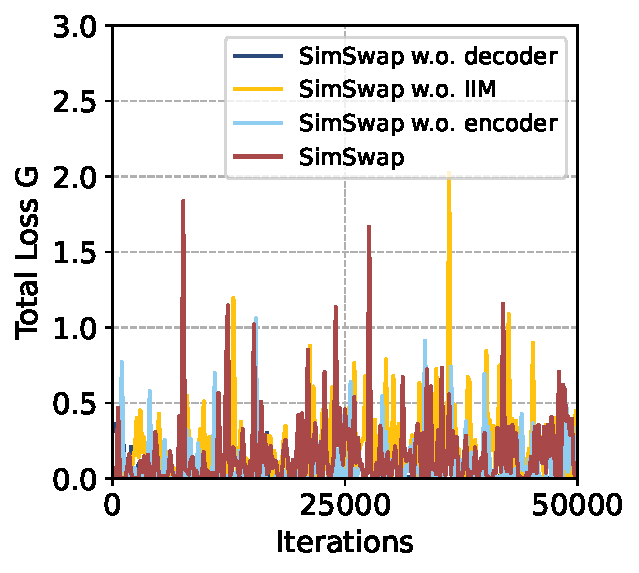
\includegraphics[scale=0.42]{real.pdf}
    }

\caption{Change of Loss D in Ablation Studies of Net G}
\label{lossD-G}
\end{figure*}

\textbf{2. Reconstruction Loss}

由图\ref{rec}可见,整体而言,移除了IIM后重建损失最小,其次是原版的SimSwap;移除encoder或decoder后重建损失均较大。

重建损失对比的是换脸目标和换脸结果,而移除IIM后生成的图片基本上就是换脸目标的原图,因此移除IIM后重建损失当然最小。而移除decoder或encoder均导致重建损失一定程度上升,体现decoder和encoder相对简单的缩放操作而言能更好地提取关键特征并重建图像。

\vspace{1.5em}
\textbf{3. wFM Loss}

由图\ref{wFM}可见,整体而言,移除IIM后弱特征匹配损失最小,其次是原版的SimSwap。

wFM Loss的目的是衡量换脸目标中非脸部的特征保持程度,由于移除IIM后生成的图像即为原图,该消融实验的wFM Loss在四个实验中最小是合理的。

移除Encoder和Decoder部分后wFM Loss上升,可见这两部分对换脸目标中非脸部信息的保持和重建也有重要作用。

\subsubsection{LossD: Net D上的整体损失}

四个实验中Net D上的Loss大小基本上一致。

由于笔者只对Net G部分进行了消融实验,四个实验的Net D部分都是一样的,这一结果是合理的。

\subsubsection{换脸结果对比}

四个实验的换脸结果在附录中的图\ref{fig-G}和图\ref{fig-loss}中分别展示。

原本SimSwap在50000轮训练已经完成到了一些特征的迁移(如图\ref{app0}中右上图对眼睛形状进行了修改,瞳色变化且眼睛下方的卧蚕变得明显,左下图中将眼睛形状修改为扁长的眼型,瞳仁颜色也有变化)。

移除encoder部分(换用缩放)后,依然可以看出换脸源到换脸目标中的特征的迁移(图\ref{app1}中右上图对瞳色进行了修改且改变了眼睛的形状,左下图将眼睛形状变为了下垂眼且加深了瞳色),但是相对SimSwap而言,修改有些“过度”、“不真实”,边界非常僵硬。

移除IIM部分后,图片基本与原图保持一致(如图\ref{app2})。由于IIM是换脸源到换脸目标条件信息注入的重要部分,这一结果非常符合预期。

移除decoder部分(换用缩放)后,图像的重建基本是灾难。不仅颜色发生了偏移(这一点应该是因为消融实验中强行选择了512个通道中的前三个通道予以保留,保留的信息有些不足的原因),而且图像非常模糊。decoder是图像的重建步骤,因此这一结果也符合预期。

\subsection{Loss范数的消融实验结果}

根据\textbf{1.5}中的设计,将wFM Loss和Id Loss换用L2范数后,损失函数的变化情况如图\ref{loss-l2}(见下页)。由于换范数之后,损失函数的大小肯定不一样,因此将两者放在同一张图中对比是无意义的。但查看两者loss G(图中的深红色折线)的变化趋势可以发现,换用L2范数后,损失函数的收敛速度明显变慢,而且一直处在较大的数值上缓慢下降。此外,形式没有发生变化的重建损失(Reconstruction Loss)在换用L2范数后急剧变大,几乎是使用L1范数形式Loss时重建损失的两倍。


\begin{figure*}[htb]
\centering

\subfigure[SimSwap with L1-Norm Id Loss \& wFM Loss]{\label{L1}
    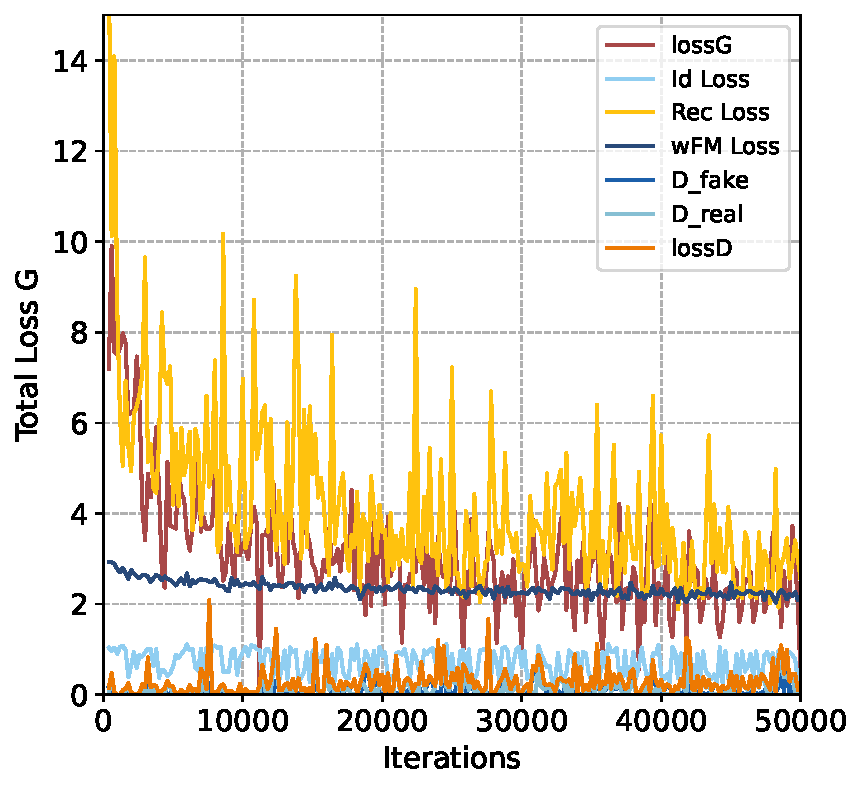
\includegraphics[scale=0.489]{L1.pdf}
    }
&
\subfigure[SimSwap with L2-Norm Id Loss \& wFM Loss]{\label{L2}
    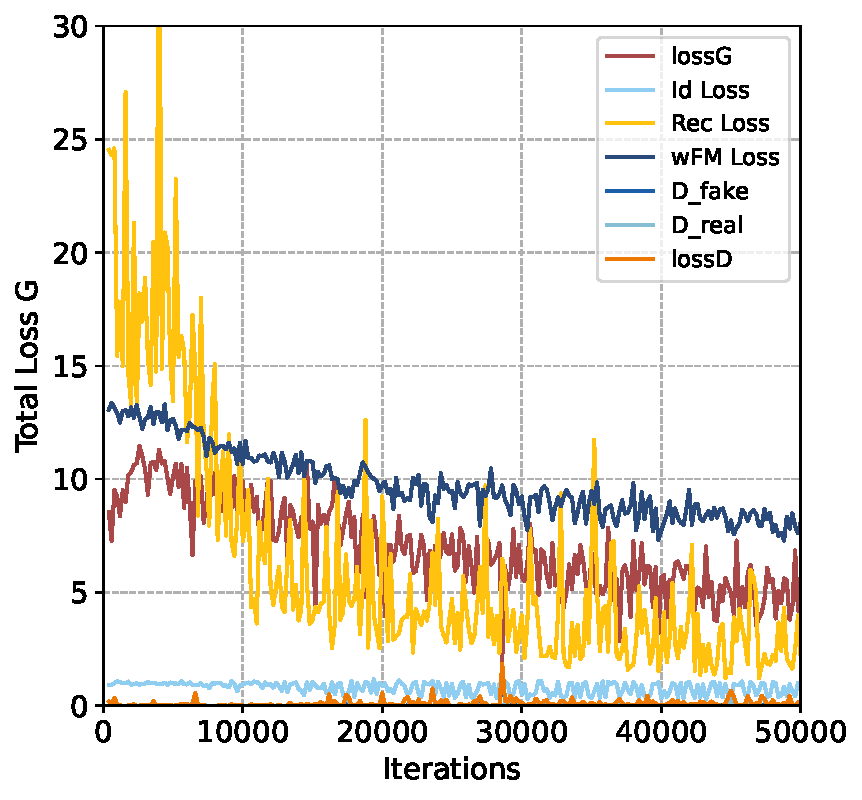
\includegraphics[scale=0.489]{L2.pdf}
    }
\caption{Change of Loss in Ablation Studies of Loss Norm}
\label{loss-l2}
\end{figure*}

对比改变Loss范数前后的换脸结果(附录图\ref{fig-loss})可以发现,使用L2范数后的换脸效果相对没有那么明显,效果略有下降。

\subsection{小结}

笔者在SimSwap的消融实验主要针对生成器(Net G)和Loss函数的形式。至于判别器(Net D)部分,由于SimSwap直接使用了已训练完毕的模型作为判别器,对其进行消融实验因此未进行进一步的消融实验。

\vspace{1em}
SimSwap的生成器(即Net G)的各个部分中,Net G的bottleneck(IMM部分)和decoder部分是最重要的两个部分。

前者负责将换脸源和换脸目标两张图片的特征信息进行融合(将源的特征信息注入到换脸目标的特征信息中),对换脸结果的影响最大,如果移除或者特征融合效果不佳,将会直接影响到换脸的效果。

后者主要负责图像的重建,因此对换脸的结果也有很大影响。

至于Net G的encoder部分,由消融实验可见,其作用其实是可以用缩放操作替代的。但是,用缩放操作提取特征会导致换脸的结果过于“硬”,发生的改变有些过度和锐化的感觉,导致换脸结果较为违和。使用多层卷积作为encoder则能使特征的变化更加“柔和”,生成的图像也相对比较真实。

\vspace{1em}
至于Loss函数(wFM Loss和Id Loss)的范数,实验证明使用L1范数能模型更快地收敛。同时,同样的训练轮数下,使用L2范数的换脸效果也不如L1范数。

\newpage

\section{VAE/GAN换脸相关论文报告}

本节为笔者对FaceShifter: Towards High Fidelity And Occlusion Aware Face Swapping\cite{faceshifter}、FSGAN: Subject Agnostic Face Swapping and Reenactment
\cite{fsgan}、DeepFaceLab: Integrated, flexible and extensible face-swapping framework\cite{deepface}三篇论文的读书报告。

\subsection{FSGAN: Subject Agnostic Face Swapping and Reenactment}

FSGAN的主要架构如图\ref{fsgan-fig},主要分为三个阶段、四个部分(对应了四个生成器)。

第一阶段包括了重演部分(rennactment)和分割部分(segmentation),对换脸源进行处理,使之尽可能接近换脸目标图片中人脸的形状,同时从两张图片中分割人脸、头发、背景区域;第二阶段包括修复部分(inpainting),根据换脸目标图片中的人脸区域,对从换脸源中分割出的人脸部分进行修复(如补充原本被头发遮挡的区域);第三阶段包括融合部分(blending),将替换后的人脸区域、换脸目标图片中的头发区域和背景区域拼接融合,从而生成换脸之后的图片。

四个生成器中,分割部分使用U-Net结构,其余三个生成器均使用pix2pixHD。

\begin{figure}[htb]
  \centering
  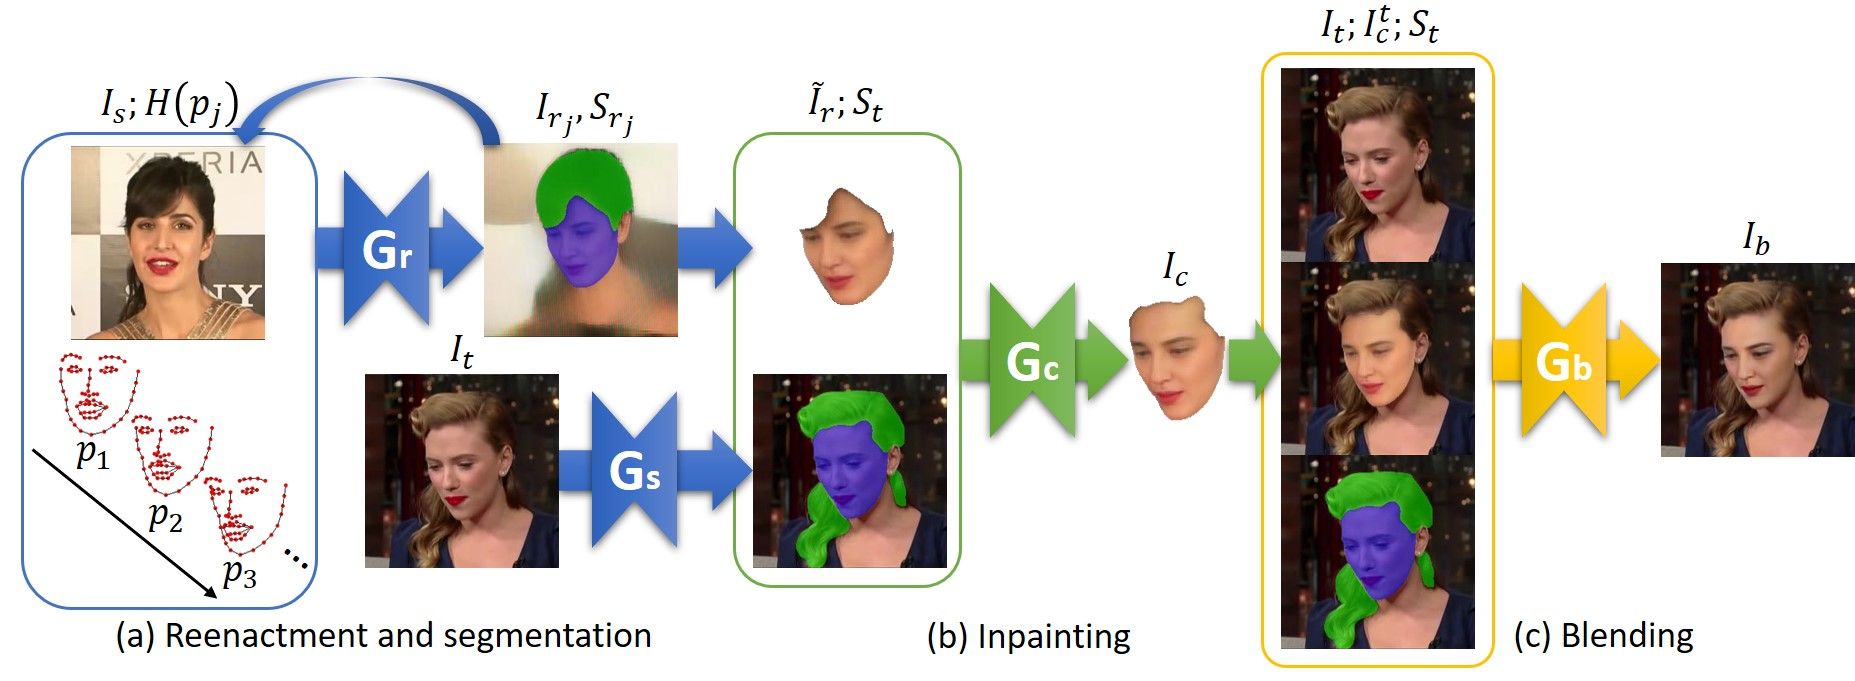
\includegraphics[width=\textwidth]{fsgan.jpg}
  \caption{An Overview of FSGAN's Generators \cite{fsgan}}
  \label{fsgan-fig}
\end{figure}

FSGAN整体的结构也可以视为一种VAE的变体。重演部分和分割部分是encoder,修复部分和融合部分可以看作decoder。修复后的换脸源的人脸信息、换脸目标图片的头发区域和背景区域相当于是两张图片的特征信息,通过融合部分这一decoder进行重建。

FSGAN的重建损失并没有使用L2范数的形式,而是用perceptual loss与逐像素的L1 loss的和来构建重建损失。对抗损失使用多尺度鉴别器,主要目的是使生成的图片看起来更真实。

该论文的创新点在于:(1)虽然个人觉得它的整体架构可以看作VAE的变体,但该论文提出的四个部分(尤其修复部分)具有参考的价值。(2)对当时来说,这篇论文应该提出了一种不错的解决用正脸源替换侧脸目标的方案(重演部分和修复部分的存在)。



\subsection{FaceShifter: Towards High Fidelity And Occlusion Aware Face Swapping}

faceshifter主要由两部分组成,第一部分AEI-net对图像进行换脸处理,第二部分HEAR NET进一步增加细节处理,还原可能在上一部分被除去的遮挡物。

AEI-net的主要结构如下图(图\ref{faceshifte}),整体依然是换脸任务很经典的encoder-decoder的结构,先从输入图片中提取特征再进行整合,然后对特征进行解码生成输出的图片。

\begin{figure}[htb]
  \centering
  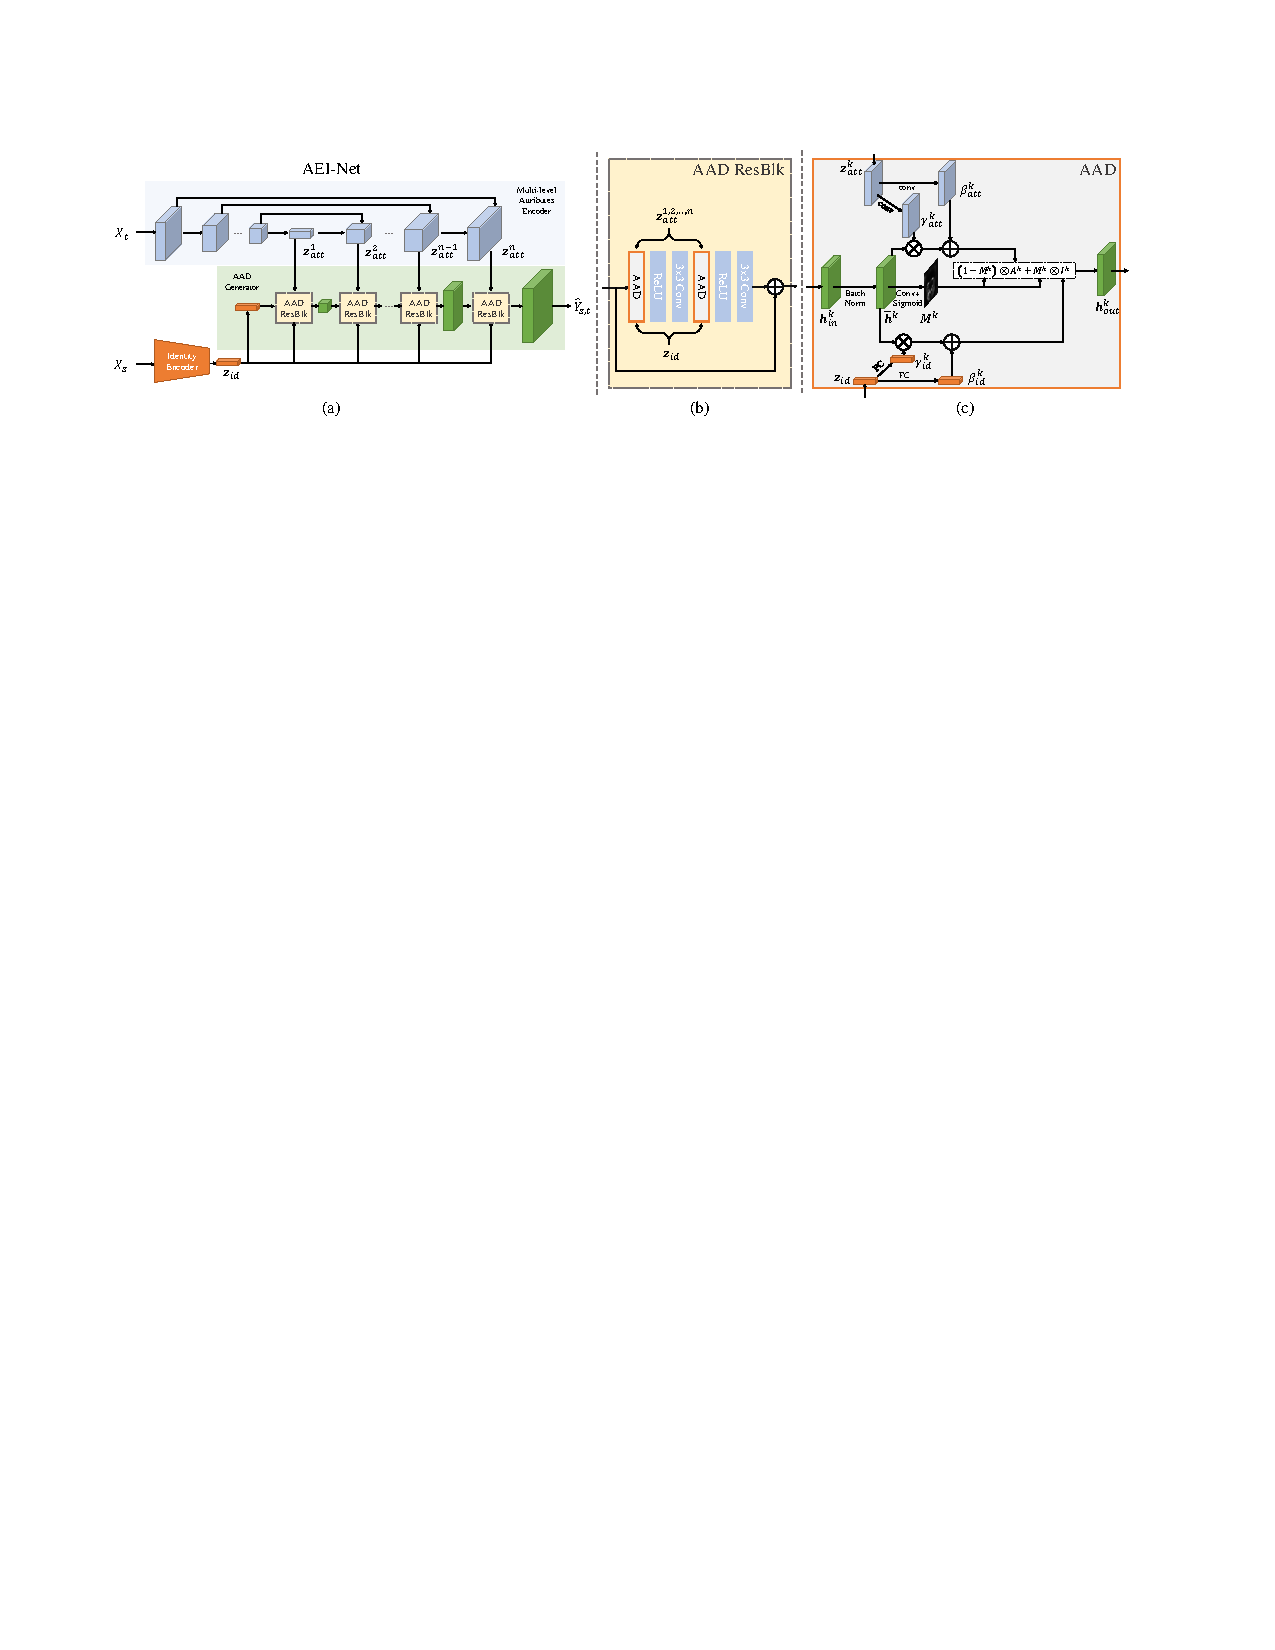
\includegraphics[width=\textwidth]{faceshifter.pdf}
  \caption{An Overview of faceshifter's AEI-Net \cite{faceshifter}}
  \label{faceshifte}
\end{figure}

AEI-Net共有三部分:Multi-level Attributes Encoder从换脸目标图像中提取特征,是一个多层的类似U-Net的结构(有可能是受到FSGAN的启发?);Identity Encoder从换脸源图像中提取身份信息相关的特征(即人脸特征),采用了已经预训练好的模型;AAD Generator整合来自两张图片的特征并生成换脸结果。

换言之,decoder部分和融合两张图片特征的过程是相互融合的,两者在同一个过程(AAD Generator)中完成。通过一点点融入换脸目标不同层的特征,能更好地对非人脸的背景特征和人脸特征进行分别处理,使最终的换脸效果更好。

该部分的损失函数由四部分构成:重建损失(用于限制最终的输出图像不要过于偏离换脸目标),实体保留损失(Id Loss,希望保留更多的换脸源的特征),属性保留损失(希望保留更多的换脸目标的特征)和对抗损失(用于使输出更加真实)。

*该论文使用的Id Loss使用余弦相似性来衡量。

\vspace{1em}
HEAR NET在AEI-Net的处理结果上进行进一步的细节处理,使用启发式方法处理面部遮挡的恢复。该部分的结构也是一个类似U-Net的结构,如图\ref{hear}。

\begin{figure}[htb]
  \centering
  \includegraphics[width=\textwidth]{hear.pdf}
  \caption{An Overview of faceshifter's HEAR-NET \cite{faceshifter}}
  \label{hear}
\end{figure}

这一部分的设计应该算是这篇论文最重要的创新点。此前的论文(包括近期的论文)基本上很少考虑换脸完成后对被“误伤”的遮挡物的处理(如发丝,帽檐等)。

该部分的损失函数由三部分组成:与AEI-Net类似的实体保留损失(Id Loss)和重建误差,以及描述经过HEAR-NET前后图片变化的损失(希望HEAR-NET尽可能少地改变图像,不要把前一阶段的换脸结果也给修改了)。

* 描述图片变化的损失也使用了L1范数。

\vspace{1em}
总结而言,faceshifter最重要的两个贡献是:(1) 提出了AAD生成器,通过多次融合换脸源的身份特征与换脸目标的不同层次特征信息的方式来达到更好的换脸效果。(2) 提出了HEAR-NET对原图中遮挡人脸的细节进行修复。这些细节很有可能在完成换脸后被“误伤”而消失,因此这一部分的提出具有很大价值。

\subsection{DeepFaceLab: Integrated, flexible and extensible face-swapping framework}

DeepFaceLab是一个著名的换脸开源项目,该论文是作者团队在2020年发布的论文,解释了DeepFaceLab的工作原理。

DeepFaceLab也是基于图像分割来完成换脸任务的,直接使用了TernausNet分割出头发、眼睛、嘴等关系到人脸特征的部分,最终分割出人脸区域。

个人认为DeepFaceLab最重要的是区域分割完成后的训练阶段(如图\ref{dfl})。其中当时比较新颖的训练方式如下(LIAE),基本也是VAE的框架。encoder和decoder部分参数共享,但在换脸源的编码过程引入了换脸目标的信息,并在融合后的特征信息重建出“换脸源”。

\begin{figure}[htb]
  \centering
  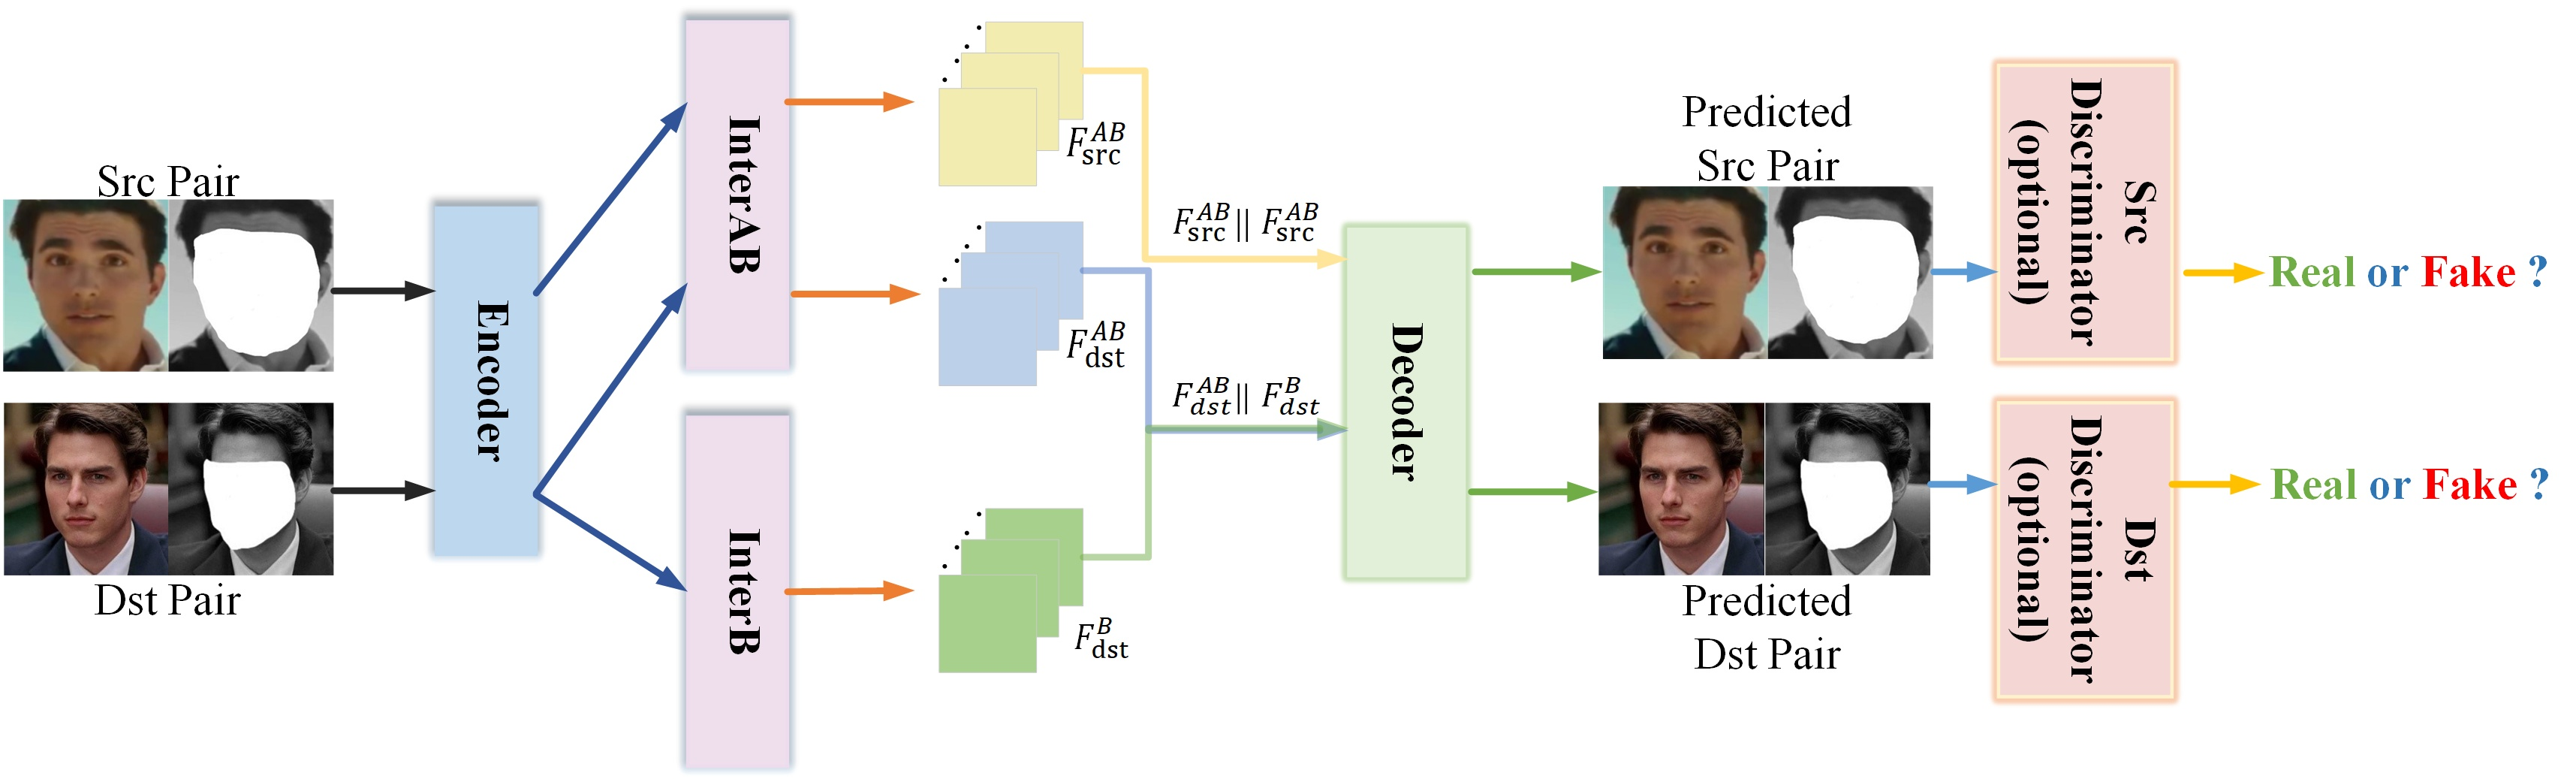
\includegraphics[width=\textwidth]{deepfacelab.jpg}
  \caption{An Overview of LIAE Structure \cite{deepfacelab}}
  \label{dfl}
\end{figure}

由于最终需要把换脸源的脸部替换到换脸目标的脸部区域中,为了使最终的结果看起来“浑然一体”,预先加入换脸目标的特征信息确实有利于换脸源在decode过程中"靠近"换脸目标的风格。LIAE的这种不平衡结构某种意义上可以看成FSGAN的“重演生成器”的变体,先将换脸源的脸部进行一些早期的变化,使之更匹配换脸目标中的脸部区域。

\vspace{1em}
之后对训练完毕得到的“换脸源”的脸部区域和“换脸目标”的非脸部区域进行对齐、修复、融合,基本中规中矩,基本没有特别的创新。

\vspace{1em}
这篇论文的最大创新点是LIAE的这种不平衡结构。这一不平衡结构提前给出了从换脸源到换脸目标的方向性,能对换脸源进行一些早期的处理。

(其实第一眼看到LIAE结构的时候就感觉这个形式非常像推荐系统中的非平衡双塔模型,也是第一层共享参数,第二层数据流非平衡地走向两个不同的模型。不太确定两者之间是否存在可以类比的关系。)


\section{Denoising Diffusion Probabilistic Models论文报告}

本节内容为Denoising Diffusion Probabilistic Models\cite{ddpm}的论文阅读报告。

\subsection{扩散模型\cite{AI2613}}

在随机过程课程中提及diffusion(连续的随机过程),其随机微分方程如下:


\vspace{-1.5em}
$$\mathrm{d}\mathbf{x}=\mathbf{f}(\mathbf{x},t)\mathrm{d}t+g(t)\mathrm{d}\mathbf{w}$$


\vspace{-1em}
($\mathbf{w}$为Brownian Motion。)

\subsection{对DDPM的整体理解}

DDPM先经过多轮加噪将原图转化为纯高斯噪声(训练),再从噪声中采样,逆向降噪得到一张生成的图像(生成)。

\begin{figure}[htb]
  \centering
  \includegraphics[width=0.8\textwidth]{ddpm.png}
  \caption{An Overview of DDPM Process \cite{ddpm}}
  \label{ddpm}
\end{figure}

我们希望最终得到的模型如图\ref{ddpm}:从噪声中采样,经过一系列模型进行降噪后,能得到一张合理的图像。某种意义上说,加噪环节类似于encode,而降噪部分则有些类似VAE的decode环节。

\subsection{DDPM的核心}

如图\ref{ddpm}所示,虽然加噪的过程$q{\mathbf{x}_t|\mathbf{x}_{t-1}}$非常容易建模(用马尔科夫链建模即可,每一步增加的噪声用高斯噪声建模),即(其中$\mathbf{z}_t\sim\mathcal{N}(\bf{0},\mathbf{1})$)

\vspace{-1em}
$$\mathbf{x}_t|\mathbf{x}_{t-1}=\sqrt{\beta_t}\mathbf{z}_t+\sqrt{1-\beta_t}\mathbf{x}_{t-1}$$

\vspace{-0.5em}
但是,降噪的过程$q(\mathbf{x}_{t-1}|\mathbf{x}_{t})$难以表示。因此DDPM使用训练神经网络的方式来建模这一降噪的过程。通过推导,得到以下重要公式:

\begin{enumerate}
    \setstretch{1.0}
    \item 扩散(加噪)过程中,从原始图片$\mathbf{x}_0$出发得到第$t$步的图像:$\mathbf{x}_t=\sqrt{\overline{\alpha}_t}\mathbf{x}_0+\sqrt{1-\overline{\alpha}_t}\mathbf{z}$
    
    其中$\alpha_t=1-\beta_t,\overline{\alpha}_t=\prod_{i=1}^t\alpha_i$.
    \item 降噪(逆向)过程中,反向的条件概率$q(\mathbf{x}_{t-1}|\mathbf{x}_{t},\mathbf{x}_0)=\mathcal{N}\left(\mathbf{x}_{t-1};\boldsymbol{\mu}(\mathbf{x}_t,\mathbf{x}_0),\hat{\beta}_t\mathbf{1}\right)$
    
    其中$\hat{\beta}_t=\frac{1-\overline{\alpha}_{t-1}}{1-\overline{\alpha}_t}\beta_t,\boldsymbol{\mu}_t=\frac{1}{\sqrt{\overline{\alpha}_t}}\left(\mathbf{x}_t-\frac{\beta_t}{\sqrt{1-\overline{\alpha}_t}}\mathbf{z}_t\right)$
\end{enumerate}


从最大化对数似然的想法出发,可以得到使用KL散度的损失函数。

\vspace{1em}
DDPM的模型结构为加入了时序嵌入模块的U-Net。(加入时序嵌入模块是因为不同时间的降噪不同,该模型应当对时间敏感。)

DDPM的训练过程与生成(采样)过程如下图。
\vspace{-1em}
\begin{figure}[htb]
  \centering
  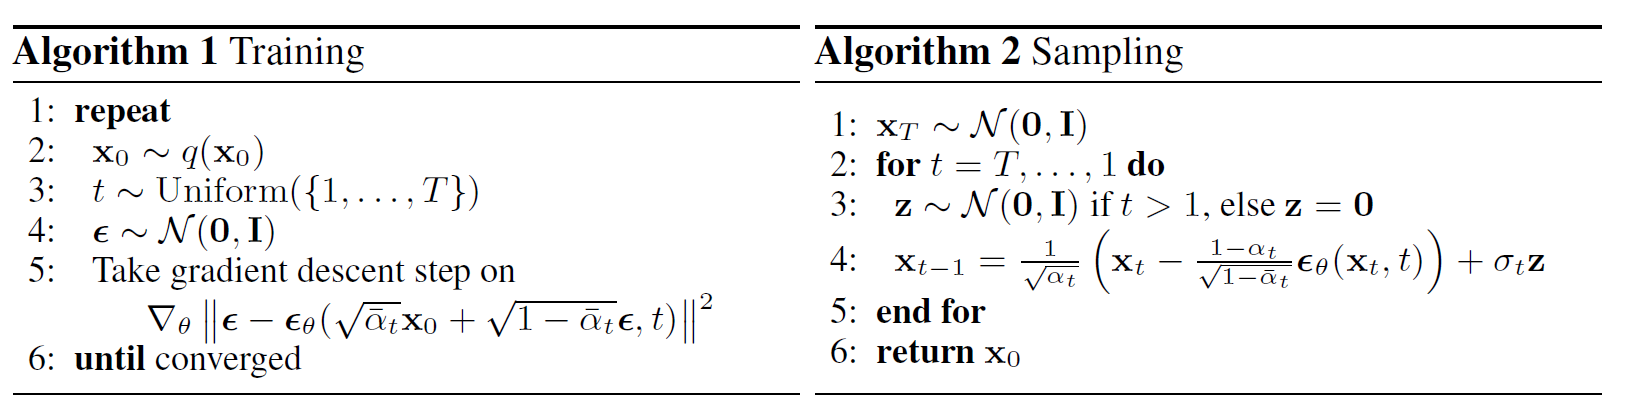
\includegraphics[width=\textwidth]{ddpm-algo.png}
  \caption{Training and Sampling of DDPM \cite{ddpm}}
  \label{ddpm-pro}
\end{figure}

\vspace{-1em}
对该模型的训练过程即为加噪过程:对时间进行随机采样并生成噪音,对图片进行加噪处理后,在原始图片、时间和加噪后的图片上训练模型拟合不同时间$t$下的“降噪”。

使用该模型生成图片的过程即降噪过程,从高斯噪声中采样,经过训练得到的模型进行降噪后,得到生成的图像。

\subsection{DDPM的创新点}

个人认为DDPM的核心思想依然是很经典的传统模型的想法,即通过一定操作(encode)将图片用潜在空间中的一个分布(DDPM为高斯噪声)表征,分布中的每一个数据点都应当对应一个图像。然后再用一系列操作(decode)将该分布中的某一个点解码为生成的图像。

DDPM的创新之处在于用随机过程(diffusion)来建模encode过程和decode过程。对难以建模的降噪过程则使用神经网络训练的方式来拟合。此外,在图像生成问题中引入时序的方法也是非常重要的创新点。

\section{特别鸣谢}
\textbf{李昱翰}助教学长。感谢助教老师对本次大作业的讲解、答疑和指导。

\textbf{樊奇}同学。SimSwap消融实验的设计与如何使用ddpm进行换脸任务方面,笔者与樊奇同学进行了一定讨论。但ddpm-swap最终的想法仍然有些问题(为了换脸把原本预训练完毕的模型再训练几次改掉的做法有些诡异)。因此最终选择读书报告的方式完成报告。

\begin{thebibliography}{}

\bibitem[1]{overview} What are Diffusion Models?, https://lilianweng.github.io/posts/2021-07-11-diffusion-models/

\bibitem[2]{simswap} SimSwap: An Efficient Framework For High Fidelity Face Swapping, \textit{R. Chen, X. Chen, B. Ni, Y. Ge}, 2020, Proceedings of the 28th ACM International Conference on Multimedia, https://arxiv.org/abs/2106.06340

\bibitem[3]{AI2619} AI2619-数字信号与图像处理,Digital Signal and Image Processing。课上的时候提到过。

\bibitem[4]{faceshifter} FaceShifter: Towards High Fidelity And Occlusion Aware Face Swapping, \textit{Lingzhi Li, Jianmin Bao, Hao Yang, Dong Chen, Fang Wen}, CVPR 2020, https://arxiv.org/abs/1912.13457

\bibitem[5]{fsgan} FSGAN: Subject Agnostic Face Swapping and Reenactment, \textit{Yuval Nirkin, Yosi Keller, Tal Hassner}, ICCV 2019, https://arxiv.org/abs/1908.05932

\bibitem[6]{deepfacelab} DeepFaceLab: Integrated, flexible and extensible face-swapping framework, \textit{Ivan Perov, Daiheng Gao, Nikolay Chervoniy, Kunlin Liu, Sugasa Marangonda, Chris Umé, Mr. Dpfks, Carl Shift Facenheim, Luis RP, Jian Jiang, Sheng Zhang, Pingyu Wu, Bo Zhou, Weiming Zhang}, https://arxiv.org/abs/2005.05535

\bibitem[7]{ddpm} Denoising Diffusion Probabilistic Models, \textit{Jonathan Ho, Ajay Jain, Pieter Abbeel}, NeurIPS 2020, https://arxiv.org/abs/

2006.11239

\bibitem[8]{AI2613} AI2613-随机过程,Stochastic Process


\end{thebibliography}

\newpage
\begin{appendix}
\section{Appendix}

\vspace{-1em}
\begin{figure*}[htb]
\centering

\subfigure[Original SimSwap]{\label{app0}
    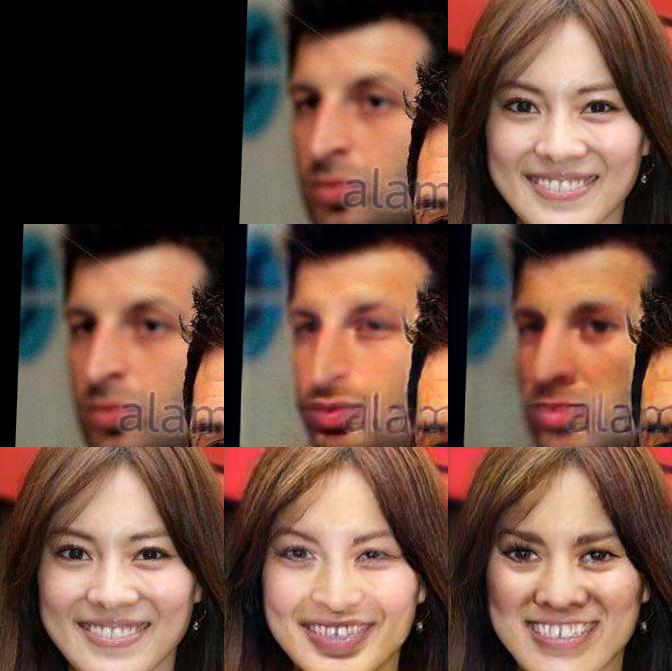
\includegraphics[scale=0.25]{orig.jpg}
    }
&
\subfigure[SimSwap without Encoder]{\label{app1}
    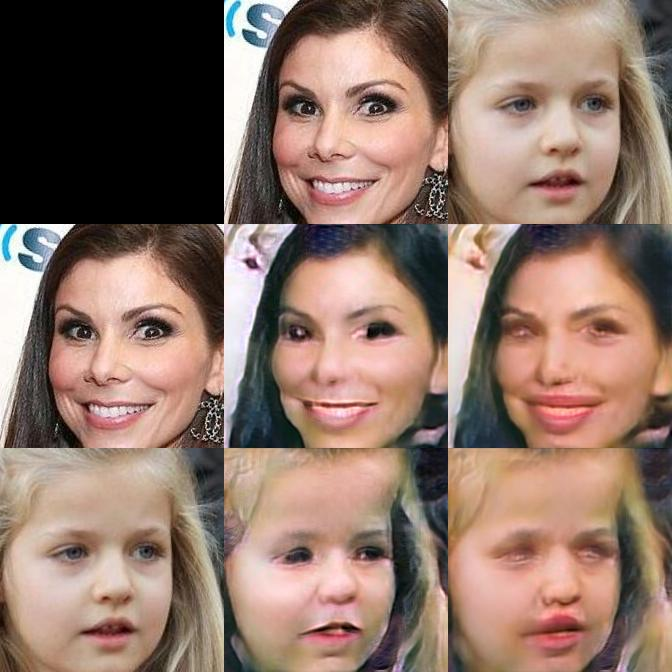
\includegraphics[scale=0.25]{no_encoder.jpg}
    }
\\
\subfigure[SimSwap without bottleneck(IIM)]{\label{app2}
    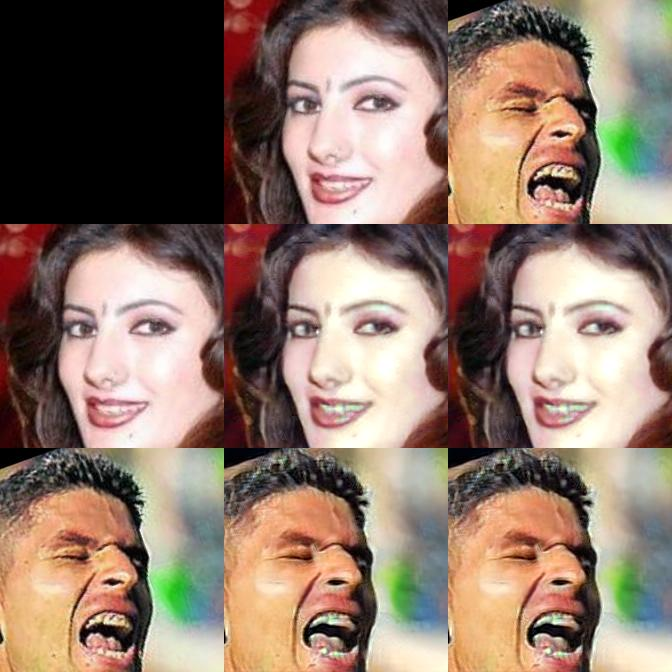
\includegraphics[scale=0.25]{no_btl.jpg}
    }
&
\subfigure[SimSwap without Decoder]{\label{app3}
    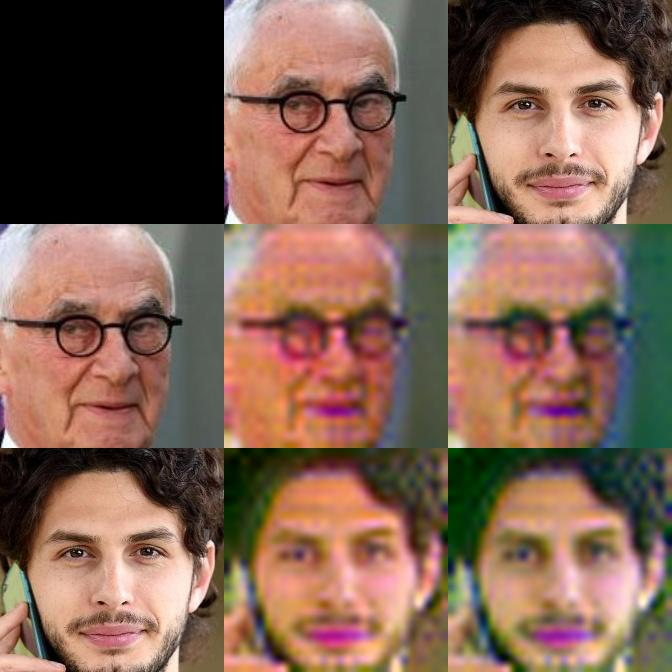
\includegraphics[scale=0.25]{no_decoder.jpg}
  }
\caption{Ablation Studies on Net G}
\label{fig-G}
\end{figure*}

\vspace{-1.5em}
\begin{figure*}[!htb]
\centering

\subfigure[Original SimSwap]{\label{app80}
    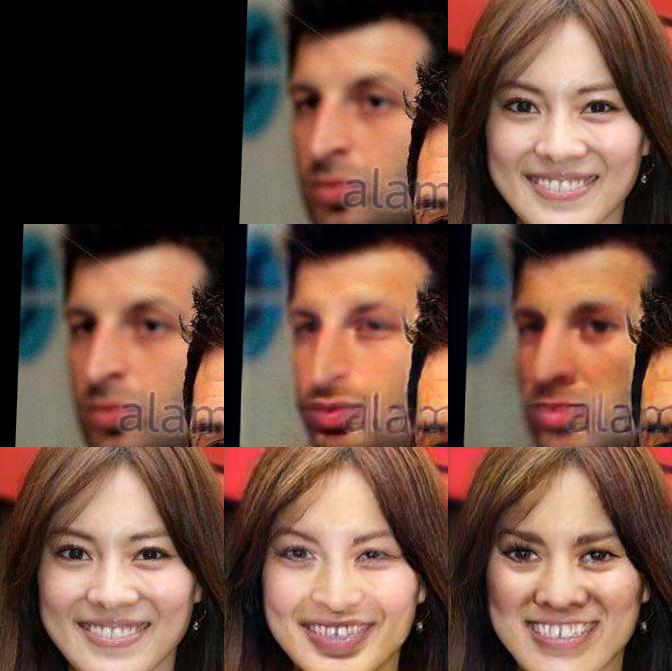
\includegraphics[scale=0.25]{orig.jpg}
    }
&
\subfigure[SimSwap with L2-Norm Recon and wFM Loss]{\label{app4}
    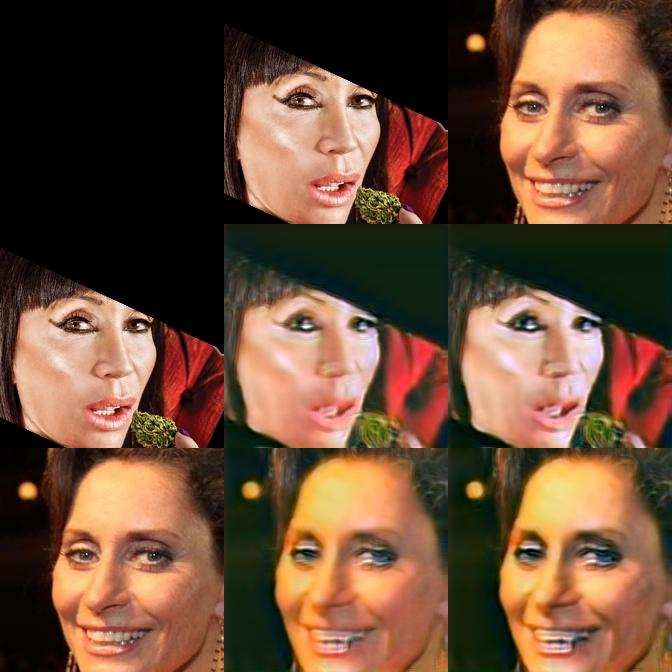
\includegraphics[scale=0.25]{abl-l2.jpg}
    }
\caption{Ablation Studies on Loss}
\label{fig-loss}
\end{figure*}



\end{appendix}

\end{document}